\chapter{Despliegue del sistema}\label{cap:despliegue}
Una vez desarrollado el sistema, es necesario desplegarlo en un servidor para que los usuarios de la UGR puedan hacer uso de él. Para ello, se ha optado por contenerizar el sistema utilizando Docker, lo que permite una fácil gestión y escalabilidad de los microservicios que componen la aplicación.
\newline\newline
El servidor en el que se despliega el sistema se encuentra en el edificio auxiliar de la ETSIIT y fue solicitado por el Departamento de Ingeniería de Computadores, Automática y Robótica. El servidor cuenta con las características técnicas definidas en el capítulo \ref{cap:planificacion}, en la sección de ``Presupuesto del proyecto''.

Además se solicitó que el servidor tuviera acceso a la red de la UGR, para que los usuarios pudieran acceder al sistema desde cualquier punto de la universidad, y que se pudiera acceder al servidor de forma remota para poder gestionar el sistema y realizar tareas de mantenimiento.
Al servidor se le ha asignado una IP privada de la red de la universidad. Por lo tanto, para acceder al servidor desde fuera de la red de la UGR, es necesario conectarse a la VPN de la universidad.

\section{Configuración del servidor}
Como paso previo a la contenerización del sistema y despliegue de la aplicación, se ha procedido a la configuración del servidor. 
\newline\newline
Esta configuración fue realizada tanto por el director como por el autor del TFG:
\begin{itemize}
    \item Creación de usuarios y grupos necesarios para el despliegue de la aplicación.
    \item Instalación de Docker y Docker Compose. Configuración de Docker para que se ejecute como servicio al iniciar el sistema.
    \item Configurar ssh para permitir el acceso remoto al servidor, y scp para la transferencia de archivos.
    \item Instalar git para poder clonar los repositorios necesarios.
\end{itemize}

No hubo más pasos previos a la contenerización del sistema, y en gran parte esta es la ventaja de contenerizar el sistema, ya que permite una fácil gestión y despliegue de la aplicación sin necesidad de realizar configuraciones complejas en el servidor.
\newline\newline
Sin hacer uso de esta tecnología se habrían tenido que realizar, entre otros, los siguientes pasos:
\begin{itemize}
    \item Configuración de un servidor web (Apache) para servir la aplicación.
    \item Configuración de un servidor de base de datos (MySQL y MongoDB) para almacenar los datos de la aplicación.
    \item Instalación y configuración de Java y Maven para compilar y ejecutar los microservicios.
    \item Instalación y configuración de Node.js y Angular CLI para compilar el frontend de la aplicación.
    \item Configuración de un servidor de mensajería (RabbitMQ) para la comunicación entre microservicios.
    \item etc
\end{itemize}

Para acceder al servidor de manera remota se ha utilizado la VPN de la UGR, que permite conectarse al servidor de forma segura y acceder a los recursos de la red de la universidad.
\newline
Y para el paso de archivos entre el servidor y el equipo local se ha utilizado el protocolo SCP (Secure Copy Protocol), que permite transferir archivos de forma segura a través de SSH.
\section{Contenerización del sistema}

El primer paso realizado en este sentido ha sido la contenerización del backend del sistema, que está compuesto por varios microservicios. 

\subsection{Pasos para la contenerización del backend}

En esta primera fase se han contenerizado, construido y levantado los servicios de la siguiente manera:

\begin{enumerate}
    \item Crear una red en docker:
    \begin{lstlisting}[language=bash]
        docker network create calendarugr
    \end{lstlisting}
    \item Generar los .jar de los microservicios, sin pasar los tests para una construcción sin conflictos para los servicios que ya están contenerizados:
    \begin{lstlisting}[language=bash]
        ./mvnw clean package -DskipTests
    \end{lstlisting}
    \item Crear las imágenes de los microservicios (Ej imagen de Eureka service):
    \begin{lstlisting}[language=bash]
        FROM amazoncorretto:21-alpine-jdk
        WORKDIR /app
        EXPOSE 8761
        COPY ./target/eureka-service-0.0.1-SNAPSHOT.jar eureka-service.jar

        ENTRYPOINT ["java", "-jar", "eureka-service.jar"]
    \end{lstlisting}
    \item Construir la imagen de docker:
    \begin{lstlisting}[language=bash]
        docker build -t eureka-service .
    \end{lstlisting}
    \item Para levantar los contenedores uno a uno (Ej levantando el contenedor de Eureka):
    \begin{lstlisting}[language=bash]
        docker run -d --name eureka-service --network calendarugr -p 8761:8761 eureka-service
    \end{lstlisting}
    \item Bajar las imágenes oficiales de mysql:8.0.41 y mongo:6.0.4, además de las imágenes de RabbitMQ:
    \begin{lstlisting}[language=bash]
        docker pull mysql:8.0.41
        docker pull mongo:6.0.4
        docker pull rabbitmq:3-management
    \end{lstlisting}
    \item Para levantar contenedores con variables de entorno (Ej levantando el contenedor de Mysql):
    \item \begin{lstlisting}[language=bash]
        docker run -p 3307:3306 --network calendarugr \
            -e MYSQL_ROOT_PASSWORD=...\
            -e MYSQL_USER=... \
            -e MYSQL_PASSWORD=... \
            -v /home/juanmi/mysql-scripts/init.sql:/docker-entrypoint-initdb.d/init.sql \
            --name mysql \
            mysql:8.0.41
    \end{lstlisting}
    \item El init.sql es un script que se ejecuta al iniciar el contenedor de Mysql, y se utiliza para crear la base de datos y las tablas necesarias para el funcionamiento del sistema. El script se encuentra en la carpeta \texttt{mysql-scripts} del proyecto.
    \begin{lstlisting}[language=sql]
        CREATE DATABASE IF NOT EXISTS DB_USER_SERVICE;
        CREATE DATABASE IF NOT EXISTS DB_SCHEDULE_CONSUMER_SERVICE;

        GRANT ALL PRIVILEGES ON DB_USER_SERVICE.* TO 'calendarugr'@'%';
        GRANT ALL PRIVILEGES ON DB_SCHEDULE_CONSUMER_SERVICE.* TO 'calendarugr'@'%';
        FLUSH PRIVILEGES;
    \end{lstlisting}
    \item Para levantar el contenedor de Mongo:
    \begin{lstlisting}[language=bash]
        docker run -d --name mongodb \
            -p 27018:27017 \
            --network calendarugr \
            -e MONGO_INITDB_ROOT_USERNAME=... \
            -e MONGO_INITDB_ROOT_PASSWORD=... \
            mongo:6.0.4
    \end{lstlisting}
\end{enumerate}

De esta manera se levantan todos los servicios uno a uno y se pueden probar de forma individual y en conjunto. Sin embargo, para facilitar el despliegue y la gestión de los microservicios, se ha optado por utilizar Docker Compose.

\subsection{Docker Compose}
Docker Compose es una herramienta que permite definir y ejecutar aplicaciones Docker multi-contenedor. Con Docker Compose, se puede definir la configuración de todos los microservicios en un único archivo \texttt{docker-compose.yml}, lo que facilita su gestión y despliegue.
\newline\newline
Este enfoque nos permite centralizar la configuración de todos los microservicios en un único archivo, lo que facilita su gestión y despliegue, de manera que:
\begin{itemize}
    \item Cada microservicio se define como un servicio en el archivo \texttt{docker-compose.yml}.
    \item Se especifican las imágenes de cada microservicio, los puertos que se exponen, las redes a las que pertenecen y las variables de entorno necesarias.
    \item Se definen las dependencias entre los servicios, lo que permite que Docker Compose gestione el orden de inicio de los contenedores.
    \item Se pueden definir volúmenes para persistir los datos de los servicios, como en el caso de MySQL y MongoDB.
\end{itemize}

De esta manera lo único que haría falta en el servidor para levantar todo el backend sería un directorio contenedor del archivo \texttt{docker-compose.yml}. Al tener este archivo referencia a las imágenes oficiales de MySql, Mongo y RabbitMQ, además de las imágenes de los servicios subidos a Docker Hub, no es necesario tener las imágenes construidas en el servidor, ya que Docker Compose se encargará de descargarlas automáticamente al levantar los servicios.

Para levantar todos los servicios definidos en el archivo \texttt{docker-compose.yml}, se puede ejecutar el siguiente comando:
\begin{lstlisting}[language=bash]
    docker-compose up -d ( -d para que se levanten en segundo plano)
\end{lstlisting}

Además para facilitar aún se han creado automatizaciones para la construcción de las imágenes y el despliegue de los microservicios, de manera que se pueden ejecutar los siguientes comandos:
\begin{lstlisting}[language=bash]
    ./build_services.sh 
    ./upload_to_hub.sh
\end{lstlisting}

Estos scripts se encargan de construir las imágenes de los microservicios y subirlas al repositorio de Docker Hub, lo que permite que se puedan desplegar en cualquier servidor con Docker instalado.

\subsection{Pasos para la contenerización del frontend}

El frontend del sistema está desarrollado en Angular y se ha decidido contenerizarlo utilizando Apache como servidor web. A continuación se detallan los pasos realizados para la dockerización del frontend:

\begin{enumerate}
    \item Construir el proyecto Angular para producción:
    \begin{lstlisting}[language=bash]
        ng build --configuration production
    \end{lstlisting}
    Este comando generará una carpeta \texttt{dist} con los archivos necesarios para desplegar la aplicación. Estos serán trasladados a un directorio del servidor, por ejemplo, \texttt{built\_tempus}, y deberá estar disponible en el mismo directorio que el docker-compose.yml, los certificados, y un directorio ``apache'' con el archivo de configuración de Apache y el Dockerfile.
    \newline
    Además, dentro del directorio \texttt{built\_tempus} se debe crear un archivo \texttt{.htaccess} con el objetivo de redirigir todas las peticiones al archivo \texttt{index.html} del frontend, para que Angular pueda manejar el enrutamiento de la aplicación. El contenido del archivo \texttt{.htaccess} es el siguiente:
    \begin{lstlisting}[language=bash]
        RewriteEngine On
        RewriteBase /
        RewriteRule ^index\.html$ - [L]
        RewriteCond %{REQUEST_FILENAME} !-f
        RewriteCond %{REQUEST_FILENAME} !-d
        RewriteRule . /index.html [L]
    \end{lstlisting}
    \item Solicitar los certificados SSL necesarios para el dominio \texttt{tempus.ugr.es}. Estos certificados son necesarios para habilitar HTTPS en el servidor web, y habilitarlo tanto para el frontend como para el backend.
    \item Copiar los certificados SSL en una carpeta del servidor, por ejemplo, en \texttt{/home/user/certificates}. Estos certificados son necesarios para habilitar HTTPS en el servidor web.
    \item Crear un archivo de configuración para Apache (\texttt{apache-ssl.conf}) en el que se especifique la configuración del servidor web.
          Aquí se especifican el uso de SSL, la redirección de HTTP a HTTPS y la configuración del \hyperlink{reverseproxy}{Reverse Proxy} para el backend.
        \begin{lstlisting}[language=bash] 
            <VirtualHost *:443>
                ServerName tempus.ugr.es
                ServerAlias xxx.xx.xxx.xxx

                # Directorio raiz donde se encuentra tu aplicacion Angular
                DocumentRoot /var/www/html

                # Habilitar SSL
                SSLEngine on
                SSLCertificateFile /ejemplo/de/ruta/certificado.pem                
                SSLCertificateKeyFile /ejemplo/de/ruta/clave-privada.pem

                # Configuracion de cifrados seguros
                SSLCipherSuite "HIGH:MEDIUM:!MD5:!RC4:!3DES"
                SSLHonorCipherOrder on

                # Protocolos seguros
                SSLProtocol -all +TLSv1.2 +TLSv1.3

                SSLProxyEngine On
                SSLProxyProtocol -all +TLSv1.2
                SSLProxyCheckPeerCN off
                SSLProxyCheckPeerName off

                # PROXY PARA EL API GATEWAY
                ProxyPass /calendarugr/v1 http://api-gateway:8090/calendarugr/v1
                ProxyPassReverse /calendarugr/v1 http://api-gateway:8090/calendarugr/v1

                <Directory /var/www/html>
                        Options Indexes FollowSymLinks
                        AllowOverride All
                        Require all granted
                    </Directory>

                    ErrorLog ${APACHE_LOG_DIR}/mi-app-error.log
                    CustomLog ${APACHE_LOG_DIR}/mi-app-access.log combined
                </VirtualHost>
        \end{lstlisting}
        Este archivo de configuración define un VirtualHost para el dominio \texttt{tempus.ugr.es} en el puerto 443 (HTTPS).
        \newline 
        Gracias a esta configuración, Apache actuará como un proxy inverso para el backend, redirigiendo las peticiones al API Gateway que se ejecuta en el contenedor de Docker.
    \item Creación del Dockerfile para el frontend, que se encargará de construir la imagen del contenedor que servirá la aplicación Angular. Este archivo irá en el mismo directorio que el archivo \texttt{apache-ssl.conf}.
        \begin{lstlisting}[language=bash]
            # Base image
            FROM ubuntu:latest

            ENV DEBIAN_FRONTEND=noninteractive

            # Install apache2
            # Install dependencies
            RUN apt-get update && apt-get install -y \
                php \
                apache2 \
                libapache2-mod-php \
                curl \
                && rm -rf /var/lib/apt/lists/*
            RUN apt-get update && apt-get install -y zip unzip git
            RUN apt-get install -y iputils-ping && apt install -y iproute2

            # Activate apache2 modules and enable SSL and proxy
            RUN a2enmod rewrite ssl proxy proxy_http && mkdir /etc/apache2/ssl
            # copy ssl files
            COPY ./apache-ssl.conf /etc/apache2/sites-available/apache-ssl.conf

            # activate the site
            RUN a2ensite apache-ssl.conf

            EXPOSE 443
        \end{lstlisting}
    \item Diseñar el archivo \texttt{docker-compose.yml} para el frontend, que incluirá la configuración del contenedor de Apache y la redirección de las peticiones al API Gateway.
    En este archivo hacemos que el contenedor del frontend use la misma red que el resto de microservicios, y que se levante el contenedor de Apache con la configuración del archivo \texttt{apache-ssl.conf}.
    \newline
    Además se especifica el volumen donde se encuentran los certificados SSL, el directorio \texttt{built\_tempus} que contiene los archivos del frontend y el archivo de configuración de Apache.

\end{enumerate}

El directorio contenedor de lo necesario para desplegar el frontend debería contener algo parecido a lo siguiente:
\begin{lstlisting}[language=bash]
    - apache-docker/
        - apache/
            - apache-ssl.conf         # Configuracion de Apache con SSL
            - DockerfileApache        # Dockerfile para construir el contenedor
        - certificados/
            - ClavePrivada.pem        # Clave privada SSL
            - Certificado.pem         # Certificado SSL
        - docker-compose.yml          # Composicion de servicios Docker
        - built_tempuis               # Carpeta donde se colocan los archivos de la app Angular
\end{lstlisting}

\section{Levantar el sistema}
Una vez que se han configurado y contenerizado todos los microservicios, se puede levantar el sistema completo utilizando Docker Compose. Para ello se debe levantar primero el backend, que es el que crea también la red de Docker necesaria para el frontend, y luego el frontend.
\newline
Con esto se consigue que el sistema esté completamente desplegado y accesible a través del dominio \texttt{tempus.ugr.es}.

\subsection{Paso del HTTP a HTTPS en las llamadas al backend}
Si sólo se levantara el backend exponiendo el puerto 8090 para las peticiones al api gateway, las peticiones al backend se realizarían a través de HTTP. Sin embargo, para que el sistema funcione correctamente y se pueda acceder a él a través del dominio \texttt{tempus.ugr.es}, es necesario que las peticiones al backend se realicen a través de HTTPS.
Para ello, se ha configurado Apache como un proxy inverso que redirige las peticiones al backend a través de HTTPS. De esta manera, las peticiones al backend se realizan a través del dominio \texttt{tempus.ugr.es} y el puerto 443, que es el puerto por defecto para HTTPS.

Ejemplo de endpoint del backend al que se accede a través de HTTP:

\lstset{inputencoding=utf8}
\begin{lstlisting}[language=bash]
http://172.25.190.139:8090/calendarugr/v1/schedule-consumer/classes-from-group
\end{lstlisting}

Ejemplo de endpoint del backend al que se accede a través de HTTPS:

\lstset{inputencoding=utf8}
\begin{lstlisting}[language=bash]
https://tempus.ugr.es/calendarugr/v1/schedule-consumer/classes-from-group
\end{lstlisting}

\subsection{Pruebas de carga en un entorno real}
Una vez todo lo necesario levantado para un funcionamiento normal del sistema, se han realizado pruebas de carga en un entorno real para comprobar el rendimiento y la escalabilidad del sistema. Estas pruebas se han realizado utilizando Locust \cite{locust}, que es una herramienta de código abierto para realizar pruebas de carga y rendimiento en aplicaciones web.
\newline\newline
Las pruebas de carga se han realizado para distintos usuarios (con una media de diez suscripciones a grupos de asignatura) solicitando la información de su calendario entero (acción más común del sistema), al endpoint \texttt{https://tempus.ugr.es/calendarugr/v1/academic-subscription/entire-calendar}.\newline
Además las solicitudes no se han hecho directamente al backend mediante llamadas http, sino que se han hecho a través del dominio \texttt{tempus.ugr.es}, que es el que se utiliza para acceder al sistema desde el navegador. Esto permite simular un uso real del sistema, ya que los usuarios acceden al sistema a través del dominio y no directamente al backend.
\newline
Sabiendo que en la UGR hay aproximadamente 60.000 estudiantes, y que el número de profesores :
\begin{itemize}
    \item Pruebas de carga con 100 usuarios concurrentes, simulando un uso normal del sistema.
    \item Pruebas de carga con 500 usuarios concurrentes, simulando un uso intensivo del sistema.
    \item Pruebas de carga con 1000 usuarios concurrentes, simulando un uso extremo del sistema.
\end{itemize}

Los parámetros que mide la herramienta son los siguientes:
\begin{enumerate}
    \item \textbf{Req.}: Número total de solicitudes realizadas.
    \item \textbf{Fails}: Número de solicitudes que han fallado.
    \item \textbf{Med(ms)}: Tiempo medio de respuesta en milisegundos.
    \item \textbf{95\%ile (ms)}: Tiempo de respuesta en el percentil 95 ( es decir, el 95\% de las solicitudes se han respondido en este tiempo o menos).
    \item \textbf{99\%ile (ms)}: Tiempo de respuesta en el percentil 99 ( es decir, el 99\% de las solicitudes se han respondido en este tiempo o menos).
    \item \textbf{Avg(ms)}: Tiempo medio de respuesta en milisegundos.
    \item \textbf{Min(ms)}: Tiempo mínimo de respuesta en milisegundos.
    \item \textbf{Max(ms)}: Tiempo máximo de respuesta en milisegundos.
    \item \textbf{Avg size(bytes)}: Tamaño medio de la respuesta en bytes.
    \item \textbf{RPS}: Solicitudes por segundo.
    \item \textbf{Fails/s}: Fallos por segundo.
\end{enumerate}

\subsubsection{Pruebas de carga con 100 usuarios concurrentes}

En esta prueba se evaluó el comportamiento del sistema bajo una carga de 100 usuarios concurrentes durante 2 minutos. Los resultados cuantitativos se resumen en la Tabla~\ref{tab:locust100}.

\begin{table}[H]
\centering
\resizebox{16cm}{!}{
\begin{tabular}{|r|r|r|r|r|r|r|r|r|r|r|}
\hline
\textbf{Req.} & \textbf{Fails} & \textbf{Med(ms)} & \textbf{95\%(ms)} & \textbf{99\%(ms)} & \textbf{Avg(ms)} & \textbf{Min(ms)} & \textbf{Max(ms)} & \textbf{Avg size(Bytes)} & \textbf{RPS} & \textbf{Fails/s} \\
\hline
4172 & 35 & 84 & 120 & 6300 & 213.04 & 1 & 7329 & 9636.47 & 32.2 & 0.1 \\
\hline
\end{tabular}
}
\caption{Resultados de la prueba de carga con 100 usuarios concurrentes.}
\label{tab:locust100}
\end{table}

\begin{figure}[H]
\centering
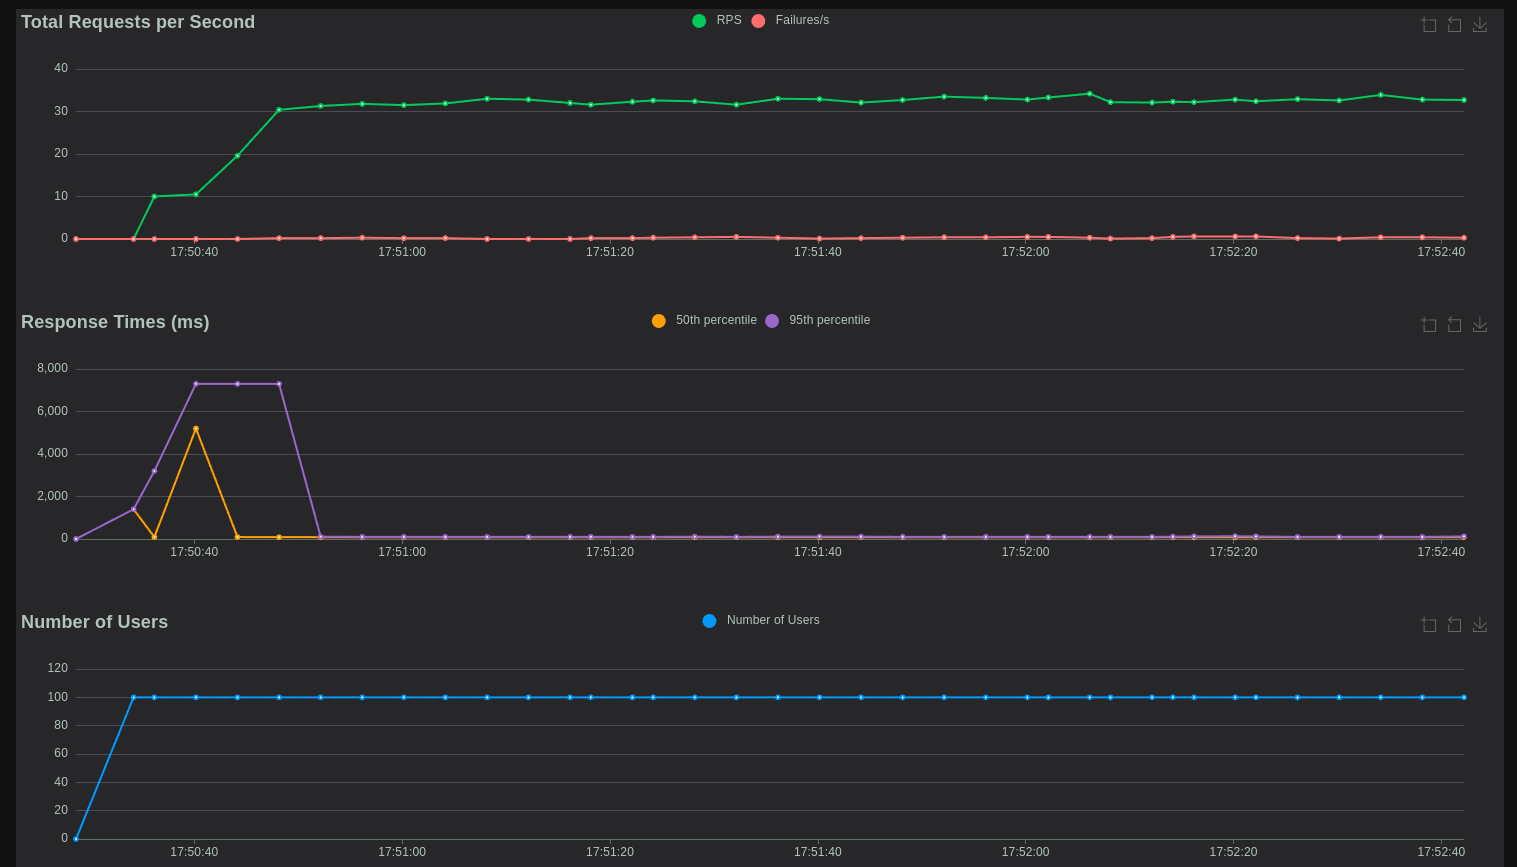
\includegraphics[width=0.9\textwidth]{figures/08_100_1.png}
\caption{Gráfica de la prueba de carga con 100 usuarios concurrentes.}
\label{fig:locust100}
\end{figure}

Del análisis de la Gráfica en la figura ~\ref{fig:locust100} y los datos de la Tabla~\ref{tab:locust100}, se extraen las siguientes observaciones:

\paragraph{Rendimiento General y Tiempos de Respuesta:}
El sistema gestionó un total de 4172 solicitudes, alcanzando un throughput promedio de 32.2 RPS. La mediana del tiempo de respuesta (Med(ms)) se situó en unos excelentes 84 ms, y el percentil 95 (95\%(ms)) en 120 ms. Estos valores indican que, una vez superada la fase inicial, la gran mayoría de los usuarios experimentaron tiempos de respuesta muy satisfactorios.
El tiempo promedio de respuesta (Avg(ms)) fue de 213.04 ms. La diferencia entre la media y la mediana sugiere la presencia de algunas latencias más elevadas, corroborado por el percentil 99 (99\%(ms)) de 6300 ms (6.3 segundos) y un tiempo máximo (Max(ms)) de 7329 ms (7.3 segundos). Aunque estos valores de cola son considerablemente más altos que el P95, afectan a un porcentaje muy reducido de peticiones bajo esta carga.

\paragraph{Comportamiento Inicial (Cold Start):}
La gráfica de ``Response Times (ms)'' (Gráfica en la figura~\ref{fig:locust100}) muestra un pico de latencia al inicio de la prueba (aproximadamente entre 17:30:00 y 17:40:00), donde el P95 alcanzó hasta 7300 ms y la mediana (P50) unos 5200 ms. Este comportamiento es característico de un ``arranque en frío'' del sistema, atribuible a factores como la carga inicial de código en el servidor de aplicaciones, el calentamiento de cachés (aplicación y base de datos PostgreSQL), la inicialización del pool de conexiones a la base de datos y el impacto de las primeras solicitudes sobre un sistema que aún no ha alcanzado su estado óptimo de operación. Tras esta fase inicial, los tiempos de respuesta se estabilizaron rápidamente a los niveles mencionados anteriormente.

\paragraph{Tasa de Fallos:}
Se registraron 35 fallos (Fails) sobre 4172 solicitudes, lo que equivale a una tasa de éxito del 99.16\% (tasa de fallo del 0.84\%). Esta tasa se considera muy baja. Los fallos fueron consistentemente del tipo \texttt{RemoteDisconnected('Remote end closed connection without response')}, sugiriendo que el servidor cerró la conexión prematuramente, posiblemente debido a timeouts durante el pico de latencia del ``cold start'' o por eventos transitorios. Dada la baja incidencia, estos fallos no señalan un problema sistémico grave bajo esta carga. El promedio de fallos por segundo fue de 0.1 Fails/s.

\paragraph{Conclusión Parcial (100 Usuarios):}
Bajo una carga de 100 usuarios concurrentes, y descontando el efecto inicial de ``cold start'', el sistema demostró ser estable y eficiente, ofreciendo tiempos de respuesta excelentes para la mayoría de las solicitudes y manteniendo una tasa de fallos mínima. Las latencias de cola (P99 y Máximo) son las primeras señales de peticiones que tardan más, pero su impacto es limitado en este nivel de carga.

\subsubsection{Pruebas de carga con 500 usuarios concurrentes}

Incrementando la carga a 500 usuarios concurrentes durante 2 minutos, se obtuvieron los resultados presentados en la Tabla~\ref{tab:locust500}.

\begin{table}[H]
\centering
\resizebox{16cm}{!}{
\begin{tabular}{|r|r|r|r|r|r|r|r|r|r|r|}
\hline
\textbf{Req.} & \textbf{Fails} & \textbf{Med(ms)} & \textbf{95\%(ms)} & \textbf{99\%(ms)} & \textbf{Avg(ms)} & \textbf{Min(ms)} & \textbf{Max(ms)} & \textbf{Avg size(Bytes)} & \textbf{RPS} & \textbf{Fails/s} \\
\hline
4918 & 48 & 88 & 280 & 15000 & 887.77 & 1 & 105514 & 9623.15 & 48.2 & 0.3 \\
\hline
\end{tabular}
}
\caption{Resultados de la prueba de carga con 500 usuarios concurrentes.}
\label{tab:locust500}
\end{table}

\begin{figure}[H]
\centering
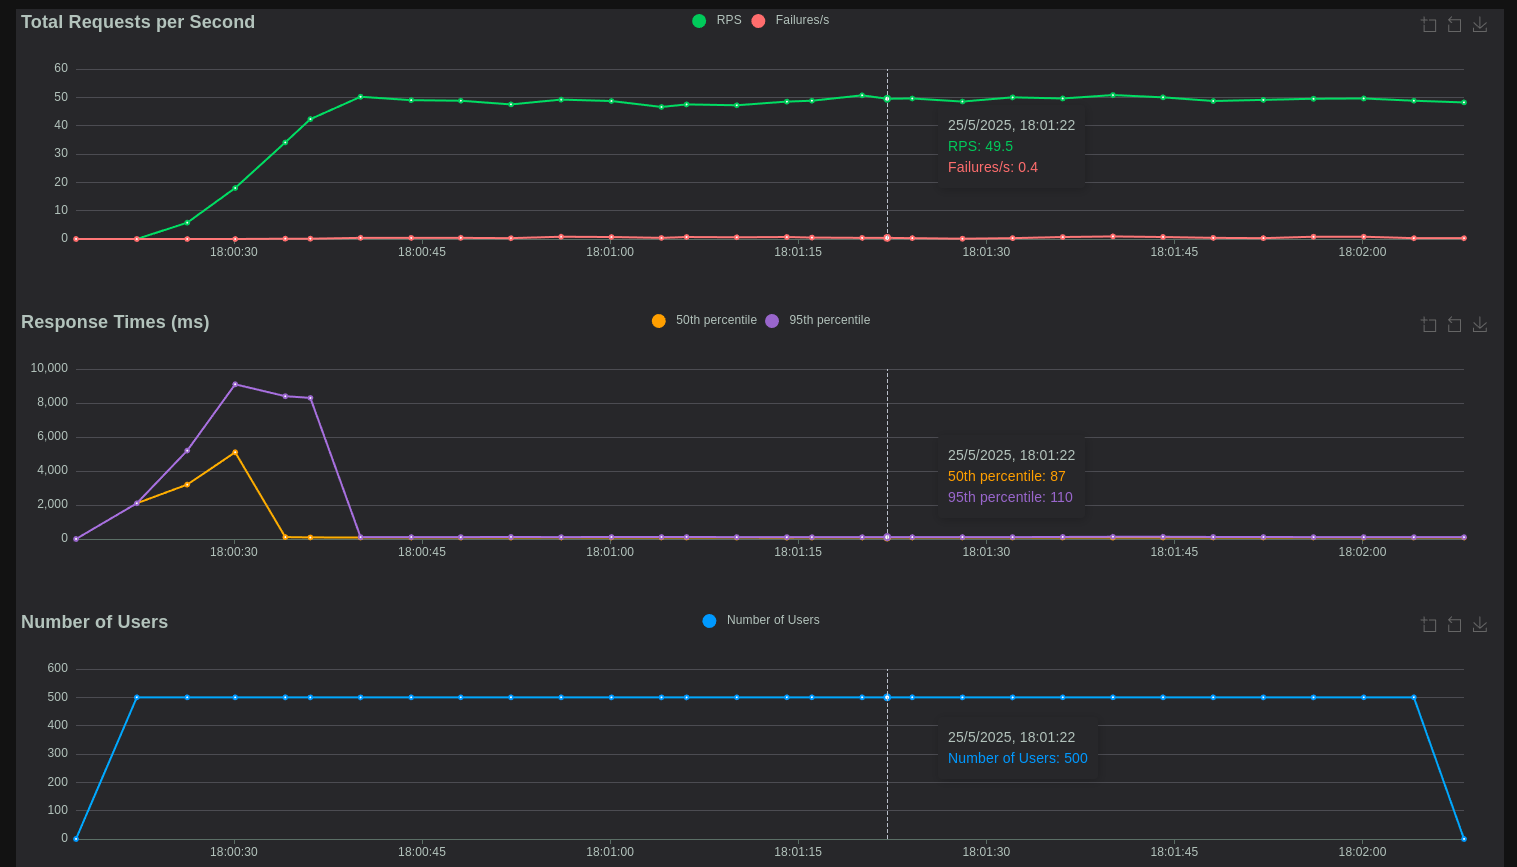
\includegraphics[width=0.9\textwidth]{figures/08_500_1.png}
\caption{Gráfica de la prueba de carga con 500 usuarios concurrentes.}
\label{fig:locust500}
\end{figure}

\paragraph{Rendimiento General y Tiempos de Respuesta:}
Con 500 usuarios, el sistema procesó 4918 solicitudes con un throughput promedio de 48.2 RPS. Es notable que, aunque el número de usuarios se quintuplicó respecto a la prueba anterior, el RPS solo aumentó aproximadamente un 50\% (de 32.2 a 48.2 RPS), lo que sugiere una disminución en la escalabilidad lineal del rendimiento.
La mediana del tiempo de respuesta (Med(ms)) se mantuvo excelente en 88 ms, similar a la prueba de 100 usuarios. Sin embargo, el P95(ms) aumentó a 280 ms, aún aceptable, pero indicando una mayor proporción de solicitudes más lentas.
El impacto en las latencias de cola es mucho más pronunciado: el P99(ms) se disparó a 15000 ms (15 segundos) y el Max(ms) a 105514 ms (105.5 segundos). Estos valores son alarmantes y evidencian que un 1-5\% de las solicitudes experimentan degradaciones severas. El Avg(ms) de 887.77 ms está fuertemente influenciado por estas latencias extremas.

\paragraph{Comportamiento Inicial (Cold Start):}
La Gráfica en la figura~\ref{fig:locust500} también muestra un pico de latencia inicial (P95 hasta 9100 ms, P50 hasta 5100 ms), atribuible al ``cold start'', similar al observado con 100 usuarios. Tras esta fase, los tiempos para la mayoría de las solicitudes (mediana) se estabilizaron.

\paragraph{Tasa de Fallos:}
Se registraron 48 fallos (Fails) sobre 4918 solicitudes, resultando en una tasa de éxito del 99.02\% (tasa de fallo del 0.98\%). Esta tasa sigue siendo baja, aunque ligeramente superior a la prueba con 100 usuarios. El promedio de fallos por segundo fue de 0.3 Fails/s.

\paragraph{Conclusión Parcial (500 Usuarios):}
Con 500 usuarios concurrentes, el sistema mantiene una buena mediana de tiempo de respuesta, pero muestra signos claros de estrés en las latencias de cola (P99 y Máximo). La escalabilidad del throughput no es lineal. Aunque la tasa de fallos es baja, la degradación severa para un pequeño porcentaje de solicitudes es un indicador de que el sistema se acerca a sus límites de capacidad o presenta cuellos de botella específicos que se manifiestan con mayor carga.

\subsubsection{Pruebas de carga con 1000 usuarios concurrentes}

La prueba final se realizó con 1000 usuarios concurrentes durante 2 minutos. Los resultados se detallan en la Tabla~\ref{tab:locust1000}.

\begin{table}[H]
\centering
\resizebox{16cm}{!}{
\begin{tabular}{|r|r|r|r|r|r|r|r|r|r|r|}
\hline
\textbf{Req.} & \textbf{Fails} & \textbf{Med(ms)} & \textbf{95\%(ms)} & \textbf{99\%(ms)} & \textbf{Avg(ms)} & \textbf{Min(ms)} & \textbf{Max(ms)} & \textbf{Avg size(Bytes)} & \textbf{RPS} & \textbf{Fails/s} \\
\hline
6672 & 215 & 92 & 2500 & 89000 & 2829.37 & 5 & 135196 & 9404.85 & 50.1 & 0.6 \\
\hline
\end{tabular}
}
\caption{Resultados de la prueba de carga con 1000 usuarios concurrentes.}
\label{tab:locust1000}
\end{table}

\begin{figure}[H]
\centering
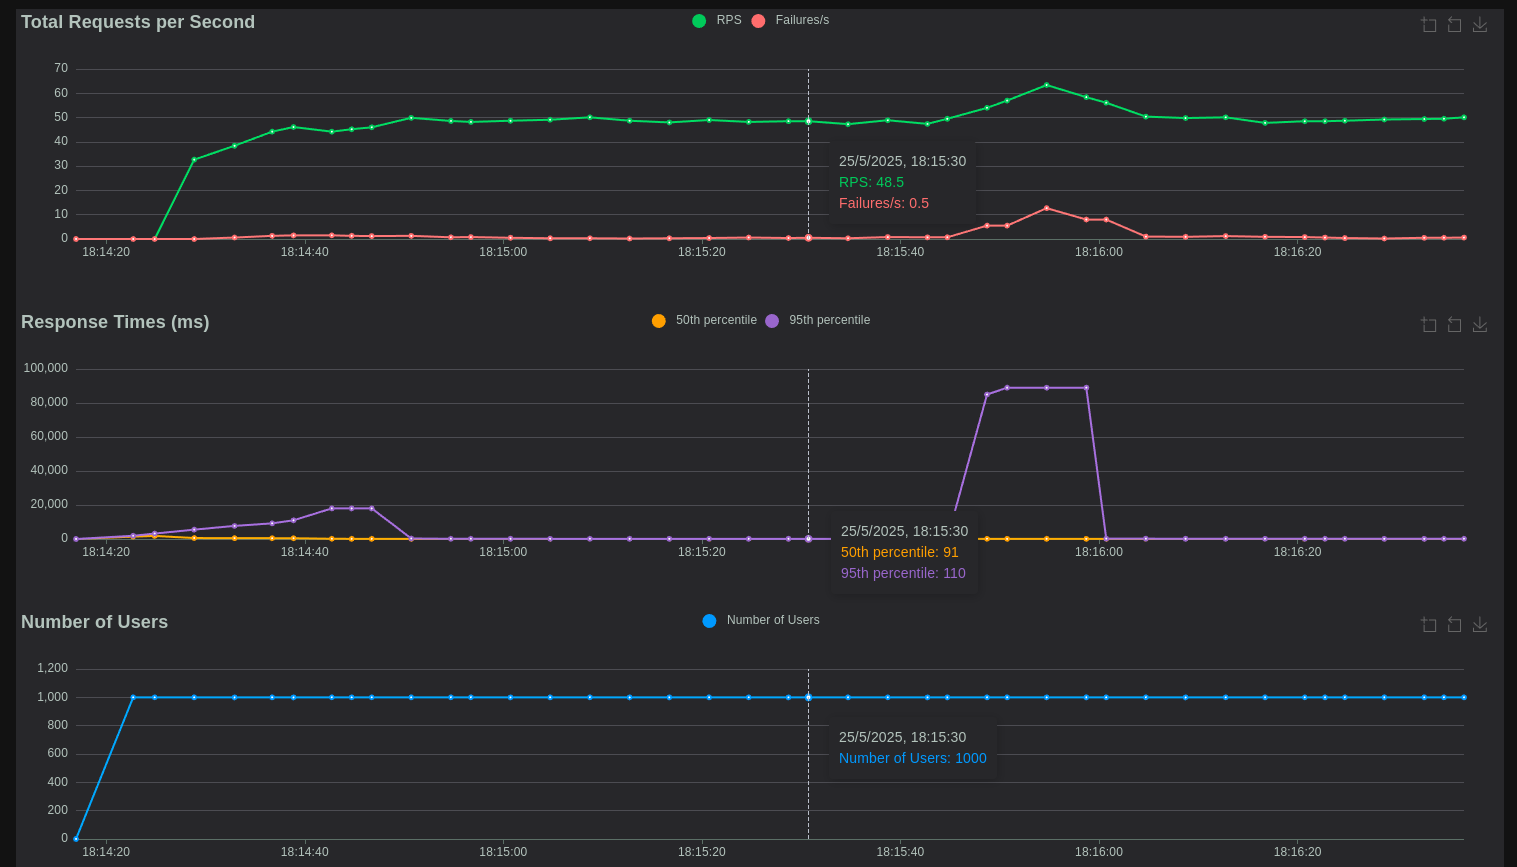
\includegraphics[width=0.9\textwidth]{figures/08_1000_1.png}
\caption{Gráfica de la prueba de carga con 1000 usuarios concurrentes.}
\label{fig:locust1000}
\end{figure}

\paragraph{Rendimiento General y Tiempos de Respuesta:}
Bajo esta carga intensiva, el sistema procesó 6672 solicitudes, con un throughput promedio de 50.1 RPS. Es crítico observar que duplicar los usuarios de 500 a 1000 apenas incrementó el RPS (de 48.2 a 50.1 RPS), lo que indica que el sistema ha alcanzado un techo de rendimiento o está operando muy cerca de su capacidad máxima.
La mediana (Med(ms)) se mantiene sorprendentemente baja en 92 ms. No obstante, este dato es engañoso si se considera aisladamente. El P95(ms) se degradó drásticamente a 2500 ms (2.5 segundos), un valor que ya impacta negativamente la experiencia del usuario. Las latencias de cola son extremas: el P99(ms) alcanzó los 89000 ms (89 segundos) y el Max(ms) los 135196 ms (135.2 segundos). Estos tiempos son indicativos de un sistema sobrecargado. El Avg(ms) de 2829.37 ms refleja el fuerte impacto de estas latencias extremas.

\paragraph{Comportamiento Inicial y Durante la Prueba:}
Se observa el pico de ``cold start'' (P95 hasta 18000 ms), aunque la mediana durante este pico inicial se mantuvo más contenida (140 ms) en comparación con los P95. Un comportamiento anómalo destacado en la Gráfica de la figura~\ref{fig:locust1000} ocurrió alrededor de los 90 segundos de prueba, donde el P99 se disparó hasta los 89000 ms. Esto sugiere un evento de saturación o un problema severo que afectó a un pequeño porcentaje de solicitudes de manera aguda durante la ejecución de la prueba, y no solo al inicio.

\paragraph{Tasa de Fallos:}
Se registraron 215 fallos (Fails) sobre 6672 solicitudes, elevando la tasa de fallo al 3.22\% (tasa de éxito del 96.78\%). Aunque no es masiva, esta tasa es significativamente superior a las pruebas anteriores y, combinada con las latencias extremas, indica problemas de estabilidad. El promedio de fallos por segundo fue de 0.6 Fails/s.

\paragraph{Conclusión Parcial (1000 Usuarios):}
Con 1000 usuarios concurrentes, el sistema está claramente sobrecargado. A pesar de una mediana de respuesta aparentemente buena, el P95 es deficiente y los P99 y Máximo son inaceptables, indicando que una proporción no despreciable de usuarios experimentaría tiempos de espera muy prolongados. El throughput se ha estancado, y la tasa de fallos, aunque no catastrófica, es una señal de alerta. El sistema no es capaz de manejar esta carga de forma eficiente ni estable. Las posibles causas de esta saturación incluyen:
\begin{itemize}
    \item \textbf{Saturación de recursos del servidor:} Límites de CPU, memoria, I/O, o descriptores de fichero en el servicio de aplicación.
    \item \textbf{Cuellos de botella en la base de datos:} Agotamiento del pool de conexiones, contención de bloqueos (locks), consultas lentas bajo concurrencia, o límites de recursos (CPU, RAM, IOPS) en PostgreSQL.
    \item \textbf{Agotamiento de recursos de red:} Posible saturación del ancho de banda o límites en el número de conexiones concurrentes a nivel de sistema operativo o balanceador de carga.
    \item \textbf{Límites de autoescalado no alcanzados o ineficaces:} Si el sistema cuenta con autoescalado, este podría no estar respondiendo con la suficiente rapidez o podría haber alcanzado sus límites configurados.
\end{itemize}

\subsubsection{Conclusiones de las Pruebas de Carga}
Las pruebas de carga progresiva con 100, 500 y 1000 usuarios concurrentes han proporcionado información valiosa sobre el comportamiento y los límites del sistema:

\begin{itemize}
    \item \textbf{Carga Baja (100 Usuarios):} Tras la fase de calentamiento inicial (``cold start''), el sistema opera de forma óptima, con tiempos de respuesta excelentes para la mayoría de las solicitudes (Mediana 84 ms, P95 120 ms) y una tasa de fallos muy baja (0.84\%). El throughput promedio fue de 32.2 RPS.
    \item \textbf{Carga Moderada (500 Usuarios):} El sistema mantiene una buena respuesta para la mayoría de los usuarios (Mediana 88 ms), pero comienzan a emerger problemas significativos en las latencias de cola (P99 de 15 segundos, Máximo de 105.5 segundos). El throughput aumentó a 48.2 RPS, pero la escalabilidad no es lineal, sugiriendo la aparición de cuellos de botella. La tasa de fallos (0.98\%) se mantiene baja.
    \item \textbf{Carga Alta (1000 Usuarios):} El sistema muestra signos evidentes de saturación. Aunque la mediana de respuesta (92 ms) puede parecer aceptable, el P95 (2.5 segundos) es deficiente y el P99 (89 segundos) y Máximo (135.2 segundos) son críticos. El throughput apenas aumenta a 50.1 RPS, indicando un techo de rendimiento. La tasa de fallos se incrementa al 3.22\%. El sistema no maneja esta carga de manera efectiva.
\end{itemize}

En resumen, el sistema es robusto y eficiente bajo cargas bajas. A medida que la concurrencia aumenta a 500 usuarios, se observan las primeras señales de estrés, principalmente en las solicitudes más lentas. Con 1000 usuarios, el sistema está sobrecargado, manifestando una degradación severa en los tiempos de respuesta para un porcentaje significativo de las solicitudes y un estancamiento del throughput.

Para mejorar la capacidad del sistema de manejar cargas más altas y optimizar su rendimiento general, se proponen las siguientes líneas de actuación:

\begin{itemize}
    \item \textbf{Análisis Profundo de Cuellos de Botella:} Utilizar herramientas de profiling y monitorización avanzada (APM) en el servidor de aplicaciones y en la base de datos para identificar los cuellos de botella exactos que causan la degradación del P99 y el estancamiento del RPS bajo cargas de 500 y 1000 usuarios. Investigar específicamente las consultas lentas, el uso de CPU/Memoria/IO y la contención de locks.
    \item \textbf{Optimización de la Base de Datos (PostgreSQL):}
        \begin{itemize}
            \item Revisar y optimizar las consultas más frecuentes o lentas identificadas en el análisis.
            \item Asegurar la correcta definición y uso de índices.
            \item Ajustar la configuración de PostgreSQL (ej. \texttt{shared\_buffers}, \texttt{work\_mem}, \texttt{max\_connections}, configuración del pool de conexiones) para la carga esperada.
        \end{itemize}
    \item \textbf{Optimización del Servidor de Aplicaciones:}
        \begin{itemize}
            \item Ajustar la configuración del servidor (ej. tamaño del heap de la JVM si es Java, número de workers/threads) para optimizar el uso de recursos.
            \item Revisar el código de la aplicación en busca de ineficiencias, especialmente en las rutas críticas o aquellas que muestran mayor latencia.
        \end{itemize}
    \item \textbf{Estrategias de Caché:} Implementar o mejorar las estrategias de caché a diferentes niveles (ej. caché de datos de aplicación con Redis o Memcached, caché de consultas de base de datos) para reducir la carga sobre los componentes más lentos, especialmente la base de datos.
    \item \textbf{Escalabilidad Horizontal y Balanceo de Carga:} Si no está implementado, considerar una arquitectura de escalado horizontal con un balanceador de carga para distribuir las solicitudes entre múltiples instancias de la aplicación. Si ya existe, revisar la configuración del balanceador y la eficiencia del autoescalado.
    \item \textbf{Revisión de Timeouts y Configuración de Red:} Ajustar los timeouts a nivel de aplicación, servidor web y balanceador de carga para evitar cierres prematuros de conexión, especialmente bajo carga, sin enmascarar problemas de rendimiento subyacentes.
\end{itemize}
La implementación de estas mejoras debería ser seguida por nuevas pruebas de carga para validar su efectividad y asegurar que el sistema puede escalar de manera eficiente y estable a mayores niveles de concurrencia.

\subsection{Solución a la sincronización con Google Calendar}

Nuestro servidor cuenta con una IP privada dentro de la red de la UGR, por lo que no es accesible desde el exterior de la red sin VPN. Esto supone un problema para la sincronización con Google Calendar, ya que este servicio requiere que el servidor sea accesible desde Internet para poder sincronizar el calendario de los usuarios con Google Calendar.
\newline\newline
Para solucionar este problema, Francisco Manuel Illeras García, profesor titular de la ETSIIT perteneciente al departamento de Ingeniería de Computadores, Automática y Robótica, ha configurado un Reverse Proxy en su servidor con IP pública que redirige las peticiones asociadas a obtener la url de sincronización con Google Calendar a nuestro servidor. De esta manera, cuando un usuario solicita la sincronización con Google Calendar, la petición se redirige al servidor de Francisco Manuel Illeras García, que a su vez redirige la petición a nuestro servidor. Esto permite que los usuarios puedan sincronizar sus calendarios con Google Calendar sin necesidad de que nuestro servidor sea accesible desde fuera de la red de la UGR.